%% bare_jrnl.tex
%% V1.4b
%% 2015/08/26
%% by Michael Shell
%% see http://www.michaelshell.org/
%% for current contact information.
%%
%% This is a skeleton file demonstrating the use of IEEEtran.cls
%% (requires IEEEtran.cls version 1.8b or later) with an IEEE
%% journal paper.
%%
%% Support sites:
%% http://www.michaelshell.org/tex/ieeetran/
%% http://www.ctan.org/pkg/ieeetran
%% and
%% http://www.ieee.org/

%%*************************************************************************
%% Legal Notice:
%% This code is offered as-is without any warranty either expressed or
%% implied; without even the implied warranty of MERCHANTABILITY or
%% FITNESS FOR A PARTICULAR PURPOSE! 
%% User assumes all risk.
%% In no event shall the IEEE or any contributor to this code be liable for
%% any damages or losses, including, but not limited to, incidental,
%% consequential, or any other damages, resulting from the use or misuse
%% of any information contained here.
%%
%% All comments are the opinions of their respective authors and are not
%% necessarily endorsed by the IEEE.
%%
%% This work is distributed under the LaTeX Project Public License (LPPL)
%% ( http://www.latex-project.org/ ) version 1.3, and may be freely used,
%% distributed and modified. A copy of the LPPL, version 1.3, is included
%% in the base LaTeX documentation of all distributions of LaTeX released
%% 2003/12/01 or later.
%% Retain all contribution notices and credits.
%% ** Modified files should be clearly indicated as such, including  **
%% ** renaming them and changing author support contact information. **
%%*************************************************************************


% *** Authors should verify (and, if needed, correct) their LaTeX system  ***
% *** with the testflow diagnostic prior to trusting their LaTeX platform ***
% *** with production work. The IEEE's font choices and paper sizes can   ***
% *** trigger bugs that do not appear when using other class files.       ***                          ***
% The testflow support page is at:
% http://www.michaelshell.org/tex/testflow/



\documentclass[journal]{IEEEtran}
%
% If IEEEtran.cls has not been installed into the LaTeX system files,
% manually specify the path to it like:
% \documentclass[journal]{../sty/IEEEtran}



%\usepackage{refcheck}

% Some very useful LaTeX packages include:
% (uncomment the ones you want to load)

\usepackage{graphicx}
\usepackage{xcolor}
\usepackage{colortbl}
\usepackage{amssymb}
\usepackage{amsmath}
\usepackage{multirow}
\usepackage{booktabs}

\allowdisplaybreaks

% *** MISC UTILITY PACKAGES ***
%
%\usepackage{ifpdf}
% Heiko Oberdiek's ifpdf.sty is very useful if you need conditional
% compilation based on whether the output is pdf or dvi.
% usage:
% \ifpdf
%   % pdf code
% \else
%   % dvi code
% \fi
% The latest version of ifpdf.sty can be obtained from:
% http://www.ctan.org/pkg/ifpdf
% Also, note that IEEEtran.cls V1.7 and later provides a builtin
% \ifCLASSINFOpdf conditional that works the same way.
% When switching from latex to pdflatex and vice-versa, the compiler may
% have to be run twice to clear warning/error messages.






% *** CITATION PACKAGES ***
%
\usepackage{cite}
% cite.sty was written by Donald Arseneau
% V1.6 and later of IEEEtran pre-defines the format of the cite.sty package
% \cite{} output to follow that of the IEEE. Loading the cite package will
% result in citation numbers being automatically sorted and properly
% "compressed/ranged". e.g., [1], [9], [2], [7], [5], [6] without using
% cite.sty will become [1], [2], [5]--[7], [9] using cite.sty. cite.sty's
% \cite will automatically add leading space, if needed. Use cite.sty's
% noadjust option (cite.sty V3.8 and later) if you want to turn this off
% such as if a citation ever needs to be enclosed in parenthesis.
% cite.sty is already installed on most LaTeX systems. Be sure and use
% version 5.0 (2009-03-20) and later if using hyperref.sty.
% The latest version can be obtained at:
% http://www.ctan.org/pkg/cite
% The documentation is contained in the cite.sty file itself.






% *** GRAPHICS RELATED PACKAGES ***
%
\ifCLASSINFOpdf
  % \usepackage[pdftex]{graphicx}
  % declare the path(s) where your graphic files are
  % \graphicspath{{../pdf/}{../jpeg/}}
  % and their extensions so you won't have to specify these with
  % every instance of \includegraphics
  % \DeclareGraphicsExtensions{.pdf,.jpeg,.png}
\else
  % or other class option (dvipsone, dvipdf, if not using dvips). graphicx
  % will default to the driver specified in the system graphics.cfg if no
  % driver is specified.
  % \usepackage[dvips]{graphicx}
  % declare the path(s) where your graphic files are
  % \graphicspath{{../eps/}}
  % and their extensions so you won't have to specify these with
  % every instance of \includegraphics
  % \DeclareGraphicsExtensions{.eps}
\fi
% graphicx was written by David Carlisle and Sebastian Rahtz. It is
% required if you want graphics, photos, etc. graphicx.sty is already
% installed on most LaTeX systems. The latest version and documentation
% can be obtained at: 
% http://www.ctan.org/pkg/graphicx
% Another good source of documentation is "Using Imported Graphics in
% LaTeX2e" by Keith Reckdahl which can be found at:
% http://www.ctan.org/pkg/epslatex
%
% latex, and pdflatex in dvi mode, support graphics in encapsulated
% postscript (.eps) format. pdflatex in pdf mode supports graphics
% in .pdf, .jpeg, .png and .mps (metapost) formats. Users should ensure
% that all non-photo figures use a vector format (.eps, .pdf, .mps) and
% not a bitmapped formats (.jpeg, .png). The IEEE frowns on bitmapped formats
% which can result in "jaggedy"/blurry rendering of lines and letters as
% well as large increases in file sizes.
%
% You can find documentation about the pdfTeX application at:
% http://www.tug.org/applications/pdftex





% *** MATH PACKAGES ***
%
\usepackage{amsmath}
% A popular package from the American Mathematical Society that provides
% many useful and powerful commands for dealing with mathematics.
%
% Note that the amsmath package sets \interdisplaylinepenalty to 10000
% thus preventing page breaks from occurring within multiline equations. Use:
%\interdisplaylinepenalty=2500
% after loading amsmath to restore such page breaks as IEEEtran.cls normally
% does. amsmath.sty is already installed on most LaTeX systems. The latest
% version and documentation can be obtained at:
% http://www.ctan.org/pkg/amsmath





% *** SPECIALIZED LIST PACKAGES ***
%
%\usepackage{algorithmic}
% algorithmic.sty was written by Peter Williams and Rogerio Brito.
% This package provides an algorithmic environment fo describing algorithms.
% You can use the algorithmic environment in-text or within a figure
% environment to provide for a floating algorithm. Do NOT use the algorithm
% floating environment provided by algorithm.sty (by the same authors) or
% algorithm2e.sty (by Christophe Fiorio) as the IEEE does not use dedicated
% algorithm float types and packages that provide these will not provide
% correct IEEE style captions. The latest version and documentation of
% algorithmic.sty can be obtained at:
% http://www.ctan.org/pkg/algorithms
% Also of interest may be the (relatively newer and more customizable)
% algorithmicx.sty package by Szasz Janos:
% http://www.ctan.org/pkg/algorithmicx




% *** ALIGNMENT PACKAGES ***
%
%\usepackage{array}
% Frank Mittelbach's and David Carlisle's array.sty patches and improves
% the standard LaTeX2e array and tabular environments to provide better
% appearance and additional user controls. As the default LaTeX2e table
% generation code is lacking to the point of almost being broken with
% respect to the quality of the end results, all users are strongly
% advised to use an enhanced (at the very least that provided by array.sty)
% set of table tools. array.sty is already installed on most systems. The
% latest version and documentation can be obtained at:
% http://www.ctan.org/pkg/array


% IEEEtran contains the IEEEeqnarray family of commands that can be used to
% generate multiline equations as well as matrices, tables, etc., of high
% quality.




% *** SUBFIGURE PACKAGES ***
%\ifCLASSOPTIONcompsoc
%  \usepackage[caption=false,font=normalsize,labelfont=sf,textfont=sf]{subfig}
%\else
%  \usepackage[caption=false,font=footnotesize]{subfig}
%\fi
% subfig.sty, written by Steven Douglas Cochran, is the modern replacement
% for subfigure.sty, the latter of which is no longer maintained and is
% incompatible with some LaTeX packages including fixltx2e. However,
% subfig.sty requires and automatically loads Axel Sommerfeldt's caption.sty
% which will override IEEEtran.cls' handling of captions and this will result
% in non-IEEE style figure/table captions. To prevent this problem, be sure
% and invoke subfig.sty's "caption=false" package option (available since
% subfig.sty version 1.3, 2005/06/28) as this is will preserve IEEEtran.cls
% handling of captions.
% Note that the Computer Society format requires a larger sans serif font
% than the serif footnote size font used in traditional IEEE formatting
% and thus the need to invoke different subfig.sty package options depending
% on whether compsoc mode has been enabled.
%
% The latest version and documentation of subfig.sty can be obtained at:
% http://www.ctan.org/pkg/subfig




% *** FLOAT PACKAGES ***
%
%\usepackage{fixltx2e}
% fixltx2e, the successor to the earlier fix2col.sty, was written by
% Frank Mittelbach and David Carlisle. This package corrects a few problems
% in the LaTeX2e kernel, the most notable of which is that in current
% LaTeX2e releases, the ordering of single and double column floats is not
% guaranteed to be preserved. Thus, an unpatched LaTeX2e can allow a
% single column figure to be placed prior to an earlier double column
% figure.
% Be aware that LaTeX2e kernels dated 2015 and later have fixltx2e.sty's
% corrections already built into the system in which case a warning will
% be issued if an attempt is made to load fixltx2e.sty as it is no longer
% needed.
% The latest version and documentation can be found at:
% http://www.ctan.org/pkg/fixltx2e


%\usepackage{stfloats}
% stfloats.sty was written by Sigitas Tolusis. This package gives LaTeX2e
% the ability to do double column floats at the bottom of the page as well
% as the top. (e.g., "\begin{figure*}[!b]" is not normally possible in
% LaTeX2e). It also provides a command:
%\fnbelowfloat
% to enable the placement of footnotes below bottom floats (the standard
% LaTeX2e kernel puts them above bottom floats). This is an invasive package
% which rewrites many portions of the LaTeX2e float routines. It may not work
% with other packages that modify the LaTeX2e float routines. The latest
% version and documentation can be obtained at:
% http://www.ctan.org/pkg/stfloats
% Do not use the stfloats baselinefloat ability as the IEEE does not allow
% \baselineskip to stretch. Authors submitting work to the IEEE should note
% that the IEEE rarely uses double column equations and that authors should try
% to avoid such use. Do not be tempted to use the cuted.sty or midfloat.sty
% packages (also by Sigitas Tolusis) as the IEEE does not format its papers in
% such ways.
% Do not attempt to use stfloats with fixltx2e as they are incompatible.
% Instead, use Morten Hogholm'a dblfloatfix which combines the features
% of both fixltx2e and stfloats:
%
% \usepackage{dblfloatfix}
% The latest version can be found at:
% http://www.ctan.org/pkg/dblfloatfix




%\ifCLASSOPTIONcaptionsoff
%  \usepackage[nomarkers]{endfloat}
% \let\MYoriglatexcaption\caption
% \renewcommand{\caption}[2][\relax]{\MYoriglatexcaption[#2]{#2}}
%\fi
% endfloat.sty was written by James Darrell McCauley, Jeff Goldberg and 
% Axel Sommerfeldt. This package may be useful when used in conjunction with 
% IEEEtran.cls'  captionsoff option. Some IEEE journals/societies require that
% submissions have lists of figures/tables at the end of the paper and that
% figures/tables without any captions are placed on a page by themselves at
% the end of the document. If needed, the draftcls IEEEtran class option or
% \CLASSINPUTbaselinestretch interface can be used to increase the line
% spacing as well. Be sure and use the nomarkers option of endfloat to
% prevent endfloat from "marking" where the figures would have been placed
% in the text. The two hack lines of code above are a slight modification of
% that suggested by in the endfloat docs (section 8.4.1) to ensure that
% the full captions always appear in the list of figures/tables - even if
% the user used the short optional argument of \caption[]{}.
% IEEE papers do not typically make use of \caption[]'s optional argument,
% so this should not be an issue. A similar trick can be used to disable
% captions of packages such as subfig.sty that lack options to turn off
% the subcaptions:
% For subfig.sty:
% \let\MYorigsubfloat\subfloat
% \renewcommand{\subfloat}[2][\relax]{\MYorigsubfloat[]{#2}}
% However, the above trick will not work if both optional arguments of
% the \subfloat command are used. Furthermore, there needs to be a
% description of each subfigure *somewhere* and endfloat does not add
% subfigure captions to its list of figures. Thus, the best approach is to
% avoid the use of subfigure captions (many IEEE journals avoid them anyway)
% and instead reference/explain all the subfigures within the main caption.
% The latest version of endfloat.sty and its documentation can obtained at:
% http://www.ctan.org/pkg/endfloat
%
% The IEEEtran \ifCLASSOPTIONcaptionsoff conditional can also be used
% later in the document, say, to conditionally put the References on a 
% page by themselves.




% *** PDF, URL AND HYPERLINK PACKAGES ***
%
%\usepackage{url}
% url.sty was written by Donald Arseneau. It provides better support for
% handling and breaking URLs. url.sty is already installed on most LaTeX
% systems. The latest version and documentation can be obtained at:
% http://www.ctan.org/pkg/url
% Basically, \url{my_url_here}.




% *** Do not adjust lengths that control margins, column widths, etc. ***
% *** Do not use packages that alter fonts (such as pslatex).         ***
% There should be no need to do such things with IEEEtran.cls V1.6 and later.
% (Unless specifically asked to do so by the journal or conference you plan
% to submit to, of course. )


% correct bad hyphenation here
\hyphenation{op-tical net-works semi-conduc-tor}


\begin{document}
%
% paper title
% Titles are generally capitalized except for words such as a, an, and, as,
% at, but, by, for, in, nor, of, on, or, the, to and up, which are usually
% not capitalized unless they are the first or last word of the title.
% Linebreaks \\ can be used within to get better formatting as desired.
% Do not put math or special symbols in the title.

% ---------- Preprint Notice ----------
\onecolumn
\noindent
\textbf{Preprint Notice:} This is a preprint of an article submitted to IEEE for possible publication. \\
\copyright~[2025] [Ahmad Mustafa]. This manuscript has not been peer reviewed or accepted yet. \\
Please do not redistribute without permission of the authors.

\vspace{1cm}
\twocolumn
% -------------------------------------

\title{ReCoGNet: Recurrent Context-Guided Network for 3D MRI Prostate Segmentation}
%
%
% author names and IEEE memberships
% note positions of commas and nonbreaking spaces ( ~ ) LaTeX will not break
% a structure at a ~ so this keeps an author's name from being broken across
% two lines.
% use \thanks{} to gain access to the first footnote area
% a separate \thanks must be used for each paragraph as LaTeX2e's \thanks
% was not built to handle multiple paragraphs
%

% \author{Ahmad Mustafa, Reza Rastegar, and Ghassan AlRegib% <-this % stops a space
% }

\author{
    \IEEEauthorblockN{Ahmad Mustafa,~\IEEEmembership{Member,~IEEE}, 
                      Reza Rastegar, and Ghassan AlRegib,~\IEEEmembership{Fellow,~IEEE}}
\thanks{Ahmad Mustafa (ahmadmustafa.am@gmail.com) and Ghassan AlRegib (alregib@gatech.edu) are affiliated to the School of Electrical and Computer Engineering, Georgia Institute of Technology, Atlanta, USA.}
}

% note the % following the last \IEEEmembership and also \thanks - 
% these prevent an unwanted space from occurring between the last author name
% and the end of the author line. i.e., if you had this:
% 
% \author{....lastname \thanks{...} \thanks{...} }
%                     ^------------^------------^----Do not want these spaces!
%
% a space would be appended to the last name and could cause every name on that
% line to be shifted left slightly. This is one of those "LaTeX things". For
% instance, "\textbf{A} \textbf{B}" will typeset as "A B" not "AB". To get
% "AB" then you have to do: "\textbf{A}\textbf{B}"
% \thanks is no different in this regard, so shield the last } of each \thanks
% that ends a line with a % and do not let a space in before the next \thanks.
% Spaces after \IEEEmembership other than the last one are OK (and needed) as
% you are supposed to have spaces between the names. For what it is worth,
% this is a minor point as most people would not even notice if the said evil
% space somehow managed to creep in.



% The paper headers
\markboth{Journal of \LaTeX\ Class Files,~Vol.~14, No.~8, August~2015}%
{Shell \MakeLowercase{\textit{et al.}}: Bare Demo of IEEEtran.cls for IEEE Journals}
% The only time the second header will appear is for the odd numbered pages
% after the title page when using the twoside option.
% 
% *** Note that you probably will NOT want to include the author's ***
% *** name in the headers of peer review papers.                   ***
% You can use \ifCLASSOPTIONpeerreview for conditional compilation here if
% you desire.




% If you want to put a publisher's ID mark on the page you can do it like
% this:
%\IEEEpubid{0000--0000/00\$00.00~\copyright~2015 IEEE}
% Remember, if you use this you must call \IEEEpubidadjcol in the second
% column for its text to clear the IEEEpubid mark.



% use for special paper notices
%\IEEEspecialpapernotice{(Invited Paper)}




% make the title area
\maketitle

% As a general rule, do not put math, special symbols or citations
% in the abstract or keywords.
\begin{abstract}
Prostate gland segmentation from T2-weighted MRI is a critical yet challenging task in clinical prostate cancer assessment. While deep learning-based methods have significantly advanced automated segmentation, most conventional approaches—particularly 2D convolutional neural networks (CNNs)—fail to leverage inter-slice anatomical continuity, limiting their accuracy and robustness. Fully 3D models offer improved spatial coherence but require large amounts of annotated data, which is often impractical in clinical settings. To address these limitations, we propose a hybrid architecture that models MRI sequences as spatiotemporal data. Our method uses a deep, pretrained DeepLabV3 backbone to extract high-level semantic features from each MRI slice and a recurrent convolutional head, built with ConvLSTM layers, to integrate information across slices while preserving spatial structure. This combination enables context-aware segmentation with improved consistency, particularly in data-limited and noisy imaging conditions. We evaluate our method on the PROMISE12 benchmark under both clean and contrast-degraded test settings. Compared to state-of-the-art 2D and 3D segmentation models, our approach demonstrates superior performance in terms of precision, recall, Intersection over Union (IoU), and Dice Similarity Coefficient (DSC), highlighting its potential for robust clinical deployment.

 \end{abstract}

% Note that keywords are not normally used for peerreview papers.
\begin{IEEEkeywords}
prostate segmentation, deep learning, recurrent, convolution.
\end{IEEEkeywords}






% For peer review papers, you can put extra information on the cover
% page as needed:
% \ifCLASSOPTIONpeerreview
% \begin{center} \bfseries EDICS Category: 3-BBND \end{center}
% \fi
%
% For peerreview papers, this IEEEtran command inserts a page break and
% creates the second title. It will be ignored for other modes.
\IEEEpeerreviewmaketitle



% \section{Introduction}
% The very first letter is a 2 line initial drop letter followed
% by the rest of the first word in caps.
% 
% form to use if the first word consists of a single letter:
% \IEEEPARstart{A}{demo} file is ....
% 
% form to use if you need the single drop letter followed by
% normal text (unknown if ever used by the IEEE):
% \IEEEPARstart{A}{}demo file is ....
% 
% Some journals put the first two words in caps:
% \IEEEPARstart{T}{his demo} file is ....
% 
% Here we have the typical use of a "T" for an initial drop letter
% and "HIS" in caps to complete the first word.
% \IEEEPARstart{P}{rostate} cancer remains a significant health concern, being one of the most prevalent malignancies among men worldwide. The localization and segmentation of the prostate gland are vital for early detection, diagnosis, and treatment planning \cite{Fassia2024}. The drive for automation of segmentation and localization is fueled by the potential to streamline workflows, reduce inter-observer variability, and provide reproducible standardized results in clinical settings \cite{Iosif2021}.   Due to its superior soft-tissue contrast and non-invasive nature, Magnetic Resonance Imaging (MRI) has emerged as a vital tool in the detection and evaluation of prostate cancer and deep learning has significantly impacted the screening process for the disease by automating the interpretation of MRI data \cite{Eddardaa2021}. 

% Despite remarkable advances, there are long-standing challenges in developing robust deep learning models for prostate MRI segmentation \cite{Guliev2023}. The primary hurdle is the requirement for large, annotated datasets, as deep networks thrive on voluminous supervised training data to generalize effectively \cite{Zibo2022}. Magnetic resonance annotation is inherently labor intensive and requires expert radiologists with high levels of domain knowledge and experience \cite{Silvia2022}. Not only does this process consume time and resources, but it is also impacted by inter-reader variability and heterogeneity in imaging protocols across institutions, thus hindering the scalability of dataset collection \cite{Zibo2022, Guliev2023}. Most early efforts in prostate segmentation used 2D deep learning models due to their reduced computational and data requirements \cite{Iosif2021}. However, 2D models treat individual slices independently and thus ignore important temporal or inter-slice context present in MRI series \cite{Grana_2022}. This limitation can result in inconsistencies in adjacent slices, especially at the apex and base of the prostate, where delineation is the most difficult \cite{Justinas2016}. On the other hand, 3D segmentation networks integrate volumetric information, allowing for improved consistency and boundary definition across the prostate gland \cite{Eschen2018}. However, the enhanced performance of 3D models often comes at the cost of requiring larger annotated training datasets, making them more sensitive to the scarcity of labeled volume data \cite{Briediene2022}. To address this trade-off, hybrid approaches such as 2.5D networks have emerged, which leverage contextual information from adjacent slices while avoiding the full computational cost of 3D models \cite{Yan2018}. 


% Owing to the complex anatomy and subtle boundary distinctions within MRI data, the segmentation task is predominantly handled using deep convolutional neural networks (CNNs) and their specialized variants \cite{Kuruparan2022, jensen2019prostate, khan2019zonal ,baldeon2020adaresu}. Notably, the U-Net architecture \cite{ronneberger2015u} has become a cornerstone in biomedical image segmentation due to its symmetric encoder-decoder structure with skip connections, enabling effective feature propagation and precise segmentation outcomes. Fully 3D CNNs have also been explored for volumetric segmentation \cite{mehrtash2018automatic, to2018deep}, but they are limited by the high cost of acquiring large annotated datasets and their substantial computational demands. To better capture spatiotemporal or inter-slice correlations in MRI data, a promising direction involves the use of recurrent CNNs. Unlike traditional RNN or LSTMs that process unstructured sequential data, convolutional RNNs maintain the 2D spatial structure of inputs while modeling temporal dependencies. This provides a principled approach to treating MRI volumes as sequences of correlated slices, overcoming the limitations of conventional CNNs that treat each slice independently \cite{Grana_2022}.

% There are in addition several other strategies that have gained traction to deal with scarcity of annotaed MRI data. Transfer learning, where models pretrained on large, generic image datasets or even on cross-institutional MRI datasets, are fine-tuned on smaller labeled prostate MRI datasets, has proven effective in improving model generalization and convergence \cite{Pastore_2024}. Data augmentation techniques, such as elastic deformation, brightness adjustments, and rotations, further increase data diversity and help reduce overfitting \cite{Pastore_2024}. More recently, semi-supervised learning frameworks leverage unlabeled data by generating pseudo-labels or employing consistency regularization, yielding promising results in reducing labeling requirements without sacrificing segmentation accuracy \cite{Huisman_2023}. Federated learning approaches are also being explored to train deep learning models across multiple institutions without centralized data sharing, thereby accumulating diverse training examples while preserving patient privacy and addressing dataset heterogeneity \cite{Shiradkar}.


% Building on recent advances in medical image segmentation, we propose a hybrid network architecture for accurate 3D segmentation of the prostate in T2-weighted MRI sequences. The architecture integrates two key components: (1) a pretrained DeepLabV3 backbone \cite{chen2017rethinking}, originally developed for semantic segmentation in natural images, to extract rich spatial features; and (2) a recurrent convolutional memory module designed to capture inter-slice dependencies inherent in volumetric MRI data. This combination aims to improve segmentation performance by coupling strong spatial representations with temporal context modeling. We evaluate our approach on the publicly available PROMISE12 benchmark dataset, which consists of T2-weighted MRI sequences with expert annotations for the prostate gland. Our model consistently outperforms contemporary 2D and 3D baseline methods in terms of segmentation accuracy. Moreover, we show that the recurrent convolutional module serves as a flexible plug-in head, compatible with a range of 2D segmentation backbones, and yields consistent improvements over configurations lacking temporal modeling. Finally, we assess the robustness of our model by simulating variations in image quality and illumination across MRI slices, further demonstrating the generalizability of our approach.

% The rest of the paper is structured as follows: Section II presents a brief review of recent machine learning methods for prostate segmentation. Section III details the proposed methodology. Section IV discusses experimental results, and Section V concludes the paper.

\section{Introduction}
\IEEEPARstart{P}{rostate} cancer is the second most common cancer among men globally and remains a major cause of cancer-related morbidity and mortality \cite{Fassia2024}. Accurate segmentation of the prostate gland from Magnetic Resonance Imaging (MRI), particularly T2-weighted sequences, plays a pivotal role in diagnosis, disease stratification, biopsy planning, and therapy monitoring \cite{Eddardaa2021}. However, manual annotation of prostate boundaries in MRI is time-consuming, prone to inter-observer variability, and difficult to scale across large datasets or clinical institutions. Automated segmentation using deep learning has emerged as a promising alternative, offering consistent and efficient delineations that support decision-making in clinical workflows \cite{Iosif2021}.

Convolutional neural networks (CNNs) have been widely adopted for this task due to their strong representational capabilities and success in other biomedical imaging domains \cite{Kuruparan2022, jensen2019prostate, khan2019zonal ,baldeon2020adaresu}. Most existing approaches, however, rely on 2D CNNs that process each MRI slice independently. While computationally efficient and less demanding in terms of labeled training data, these slice-wise models fail to capture inter-slice dependencies and anatomical continuity along the superior-inferior axis of the prostate. This can lead to segmentation inconsistencies, especially at the apex and base of the gland where tissue boundaries are more ambiguous.

Volumetric segmentation models based on 3D CNNs address this limitation by processing entire image stacks, thus incorporating contextual information across slices \cite{mehrtash2018automatic, to2018deep}. Yet, this gain in spatial coherence comes at the cost of higher computational complexity in 3D convolutional kernels and larger training data size, with substantial GPU resources required to train them effectively. These requirements are difficult to satisfy in real-world medical imaging settings, where data is often limited and heterogeneous in terms of acquisition protocols, scanners, and patient populations.

Recurrent neural networks (RNNs) and Long Short-Term Memory (LSTM) networks have long been used to model sequential dependencies in applications involving time series data such as speech recognition \cite{graves2013hybrid} and natural language processing \cite{wang2018lstm}. However, traditional recurrent architectures and their variants tend to not be as effective for spatiotemporal image applications requiring the prediction of dense outputs. This is because they flatten the image at each time step into a 1D vector to be processed by their fully connected layers, thereby discarding spatial information critical for accurate reconstruction of the output. 

To address this, ConvLSTM layers have been introduced \cite{shi2015convolutional}, which replace fully connected operations with convolutional ones, enabling the network to preserve spatial structure while modeling temporal dynamics. While promising, prior work employing ConvLSTM layers in the context of biomedical image analysis typically does so within relatively shallow CNN backbones \cite{almiahi2024novel}, which may limit the quality and robustness of the extracted features, particularly in heterogeneous or noisy imaging environments.

In this work, we propose ReCoGNet, a novel hybrid segmentation model that leverages both deep pretrained spatial feature extraction and sequential memory modeling. Specifically, we treat the MRI volume as a temporally ordered sequence, where each slice corresponds to a time step. A deep pretrained DeepLabV3 backbone \cite{chen2017rethinking} is used to extract rich, multiscale semantic features from each slice, and these features are then passed to a recurrent head composed of ConvLSTM layers. The recurrent head integrates contextual cues from preceding slices to inform segmentation predictions for the current slice, enabling smoother, more anatomically consistent delineations across the volume. The use of a pretrained backbone not only accelerates convergence but also enhances robustness, as it provides high-quality representations that generalize well across patients and imaging conditions.

We evaluate our proposed method on the PROMISE12 dataset \cite{litjens2014evaluation}, a widely used benchmark for prostate MRI segmentation. To emulate real-world clinical constraints, we conduct experiments under limited supervision using only 26 annotated volumes for training. In addition to standard test-time evaluations on clean data, we assess model robustness under simulated image degradation conditions—specifically, test volumes with reduced contrast in the second half of each MRI sequence. We compare our model against several state-of-the-art 2D and 3D segmentation baselines.

Our results demonstrate that the proposed model achieves superior segmentation performance across a range of metrics, including precision, recall, Intersection over Union (IoU), and Dice Similarity Coefficient (DSC), on both clean and degraded test sets. These findings highlight the advantages of combining deep spatial feature extraction with recurrent temporal modeling, and suggest that our approach is particularly well-suited for clinical deployment in settings with limited labeled data and variable imaging quality.

The rest of the paper is structured as follows: Section II presents the related work section. The methodology is described next, followed by a description of the experiments and the evaluation setup. The results are discussed next, followed by the conclusion.

\section{Related Work}
CNNs have been the dominant approach for biomedical image segmentation applications for the last several years. Notably, the U-Net architecture \cite{ronneberger2015u} has become a cornerstone architecture due to its symmetric encoder-decoder structure with skip connections, enabling effective feature propagation and precise segmentation outcomes. Over the years, several variants of UNet have been proposed such as the Attention UNet \cite{oktay2018attention} and the UNet++ \cite{zhou2018unet++}. 

The Attention UNet adds attention gates (AGs) to the standard U-Net. These gates are applied to the skip connections to suppress irrelevant features and emphasize informative regions in the encoder feature maps before concatenation with the decoder features. The UNet++ on the other hand aims to reduce the semantic gap between encoder and decoder feature maps through intermediate convolutional blocks, thereby improving segmentation performance.

While effective, these 2D CNNs operate on individual slices independently and do not capture contextual relationships between adjacent slices in 3D MRI data. To better utilize volumetric context, 3D CNNs such as VNet \cite{milletari2016v} have been applied to prostate MRI segmentation. These models process the entire MRI volume at once, thereby capturing spatial dependencies across slices. However, 3D CNNs are significantly more computationally demanding and prone to overfitting. Additionally, memory constraints often limit input resolution or batch size, which may degrade performance in fine-grained segmentation tasks. 

To preserve spatial structure while incorporating sequential memory, Convolutional LSTM (ConvLSTM) layers were introduced by Shi et al. \cite{shi2015convolutional}. ConvLSTMs replace fully connected operations with convolutional ones, enabling the network to retain spatial correlations over time. However, many existing implementations for biomedical imaging applications embed ConvLSTM layers within relatively shallow convolutional architectures, potentially limiting the quality of feature representations.

Recent studies have shown that using deep pretrained backbones, such as ResNet or DeepLabV3 \cite{chen2017rethinking}, can significantly improve segmentation performance and generalization in low-data regimes. These models, pretrained on large natural image datasets (e.g., ImageNet or COCO), capture rich semantic features and can be fine-tuned on target medical datasets with limited supervision. However, most prostate MRI segmentation studies employing pretrained networks focus solely on spatial modeling and do not leverage temporal dependencies across slices. 

To the best of our knowledge, our work is among the first to leverage the rich feature extraction capabilities of deep pretrained convolutional backbones along with the sequential modeling capablities of the ConvLSTM layers.   


% \section{Literature Review}

% Several deep learning architectures have achieved strong performance on prostate MRI segmentation benchmarks several which that most relevant to our work are discussed. 

% U-Net and its variants, which feature encoder-decoder structures with skip connections, are widely used due to their effective feature extraction and combination capabilities \cite{Grant2019}. Advanced models incorporating residual connections, attention mechanisms, or dense connectivity further enhance feature propagation and segmentation accuracy \cite{Boca_2023}. 

% A representative study proposed attaching a recurrent convolutional head to a DeepLabV3 backbone and training the network on the widely used PROMISE12 benchmark dataset, which contains T2-weighted MRI scans annotated for the prostate gland. With just 26 patients as training data, the hybrid model consistently outperformed other competitive deep learning baselines, demonstrating superior test-time segmentation performance as measured by standardized metrics such as Dice Similarity Coefficient, precision, and recall \cite{Xu_2023}.

% Segmentation models are evaluated using standardized performance metrics, notably the Dice Similarity Coefficient (DSC), which quantifies spatial overlap between predicted and ground-truth masks \cite{Xu_2023, Papanikolaou_2023}. Additional metrics such as precision, recall, Hausdorff distance (HD), and average surface distance (ASD) are extensively reported in the literature to provide a comprehensive assessment of segmentation quality. On the PROMISE12 dataset, state-of-the-art models regularly achieve DSCs above 0.85, with leading methods exceeding 0.90, rivaling expert manual annotation \cite{Xu_2023, Wang_2019}.

% An important aspect of clinical translation is the robustness of segmentation models to variations in MRI image quality, illumination, and scanner hardware. Recent systematic reviews and benchmarking studies indicate that high-performing deep learning algorithms maintain segmentation accuracy across major MRI vendors and a range of acquisition protocols. Architectures that integrate spatiotemporal modeling, such as hybrid convolutional-recurrent networks, demonstrate enhanced resilience to noise, artifacts, and interslice intensity shifts, which are common in real-world clinical imaging datasets.

% Deep learning has revolutionized prostate MRI segmentation, moving from simple 2D CNNs to sophisticated architectures that integrate transfer learning, attention, and recurrent spatiotemporal modeling, thereby improving reliability and clinical applicability. Although challenges such as annotation scarcity and imaging heterogeneity persist, ongoing developments in semi-supervised, federated, and weakly supervised learning, along with advanced network architectures, continue to push the field forward. The promise of robust prostate gland segmentation with limited labeled data heralds wider adoption of AI-assisted tools in prostate cancer screening, reducing workload for radiologists while improving standardization and accuracy.




% In \cite{khan2019zonal}, the CNN-based semantic segmentation approach is trained and tested on the NCI-ISBI 1.5T and 3T MRI data set consisting of 40 patients. Performance evaluation based on Dice similarity coefficient (DSC) of the Deeplab-based segmentation is compared with two other CNN-based semantic segmentation techniques: FCN and PSNet. The results show that prostate segmentation using DeepLabV3+ can perform better than FCN and PSNet with an average DSC of 70.3\% in PZ and 88\% in the CG zone. This indicates the significant contribution made by the atrous convolution layer, in producing better prostate segmentation result.

% In \cite{jensen2019prostate}, the authors evaluated a two-dimensional convolutional neural network (CNN) based on the U-net architecture for segmentation of the central gland (CG) and peripheral zone (PZ) using a dataset of 40 patients (34 PCa positive and 6 PCa negative) scanned on two different MRI scanners (1.5T GE and 3T Siemens). Images were cropped around the prostate gland to exclude surrounding tissues, resampled to $0.5\times 0.5 \times 0.5$ mm voxels and z-score normalized before being propagated through the CNN. Performance was evaluated using the Dice similarity coefficient (DSC) and mean absolute distance (MAD) in a fivefold cross-validation setup. Overall performance showed DSC of 0.794 and 0.692, and MADs of 3.349 and 2.993 for CG and PZ, respectively. Dividing the gland into apex, mid, and base showed higher DSC for the midgland compared to apex and base for both CG and PZ. We found no significant difference in DSC between the two scanners. A larger dataset, preferably with multivendor scanners, is necessary for validation of the proposed algorithm; however, our results are promising and have clinical potential.


% In \cite{baldeon2020adaresu}, adapting an existing convolutional neural network architecture to a specific dataset for medical image segmentation remains a challenging task that requires extensive expertise and time to fine-tune the hyperparameters. Hyperparameter optimization approaches that automate the search have been proposed but have mainly focused on optimizing the segmentation performance. However, optimizing the network size is also important to prevent unnecessary and costly computational operations. In this paper, we present a multiobjective adaptive convolutional neural network (AdaResU-Net) for medical image segmentation that is able to automatically adapt to new datasets while minimizing the size of the network. The proposed AdaResU-Net is comprised of a fixed architecture that combines the structure of the state-of-the-art U-Net with a residual learning framework to improve information propagation and promote an efficient training. Then, a multiobjective evolutionary algorithm (MEA) that optimizes both segmentation accuracy and model size is proposed to evolve the AdaResU-Net networks with different hyperparameters. The presented model is tested on two publically available medical image datasets and compared with the U-Net. Results show that the AdaResU-Net achieves better segmentation performance with less than 30\% the number of trainable parameters. Additionally, the MEA algorithm generated configurations that are smaller and perform better or equally well than configurations generated with a Bayesian hyperparameter optimization approach.

% There is large consent that successful training of deep networks requires many thousand annotated training samples. In \cite{ronneberger2015u}, a CNN based network is proposed and training strategy that relies on the strong use of data augmentation to use the available annotated samples more efficiently. The architecture consists of a contracting path to capture context and a symmetric expanding path that enables precise localization. We show that such a network can be trained end-to-end from very few images and outperforms the prior best method (a sliding-window convolutional network) on the ISBI challenge for segmentation of neuronal structures in electron microscopic stacks. Using the same network trained on transmitted light microscopy images (phase contrast and DIC) we won the ISBI cell tracking challenge 2015 in these categories by a large margin. Moreover, the network is fast. Segmentation of a 512x512 image takes less than a second on a recent GPU. 


% A system for fast automatic needle tip and trajectory localization and visualization in MRI that has been developed and tested in the context of an active clinical research program in prostate biopsy . To the best of our knowledge, this is the first reported system for this clinical application and also the first reported system that leverages deep neural networks for segmentation and localization of needles in MRI across biomedical applications. Needle tip and trajectory were annotated on 583 T2-weighted intra-procedural MRI scans acquired after needle insertion for 71 patients who underwent transperineal MRI-targeted biopsy procedure at our institution. The images were divided into two independent training-validation and test sets at the patient level. In \cite{mehrtash2018automatic}, the authors propose a deep 3-D fully convolutional neural network model was developed, trained, and deployed on these samples. The accuracy of the proposed method, as tested on previously unseen data, was 2.80-mm average in needle tip detection and 0.98° in needle trajectory angle. An observer study was designed in which independent annotations by a second observer, blinded to the original observer, were compared with the output of the proposed method. The resultant error was comparable to the measured inter-observer concordance, reinforcing the clinical acceptability of the proposed method. The proposed system has the potential for deployment in clinical routine.


% DeepLabV3, a notable deep pretrained backbone, has demonstrated success in medical semantic segmentation tasks \cite{Amila2024}. Its use of dilated convolutions enables multi-scale contextual aggregation, which is particularly beneficial for organs with variable shape and appearance, like the prostate \cite{Ali_2024}. When coupled with recurrent convolutional heads, these models can capture both spatial detail and temporal continuity across MRI sequences, resulting in more robust and coherent prostate segmentation \cite{Grana_2022}.



\section{Methodology}

In this section, we discuss the architecture of the deep network and provide a detailed explanation of the input data and how the model is trained.

\subsection{Pretrained DeepLabV3 Backbone}
The DeepLabV3 \cite{chen2017rethinking} architecture is a widely adopted deep learning model for semantic segmentation, designed to capture multi-scale contextual information while maintaining spatial accuracy in feature representations. DeepLabV3 employs an Atrous Spatial Pyramid Pooling (ASPP) module to effectively extract features at multiple receptive field scales, addressing the challenge of segmenting objects of varying sizes within an image. Unlike conventional convolutional neural networks (CNNs) that rely on downsampling operations such as max pooling and strided convolutions—potentially leading to loss of fine spatial details—DeepLabV3 incorporates atrous (dilated) convolutions, which enable feature extraction at larger receptive fields without increasing computational cost or reducing resolution.

At the core of DeepLabV3 is the ASPP module, which consists of parallel convolutional layers with different atrous rates. This structure allows the network to capture both local and global context by processing the input feature maps at multiple scales. The ASPP module is complemented by batch normalization layers and a global average pooling branch, further enhancing the model's ability to recognize structures at different levels of granularity. The final segmentation output is generated by fusing the multi-scale features extracted by the ASPP module and passing them through a lightweight decoder, which refines spatial details for improved segmentation accuracy.

\subsection{Recurrent Convolutional Head}
The ConvLSTM block, as defined in the implementation, consists of a convolutional recurrent unit that processes a sequence of MRI slices while maintaining hidden and cell states in a structured 2D format. Traditional recurrent neural networks (RNNs) and their variants, such as LSTMs and GRUs, are well-suited for modeling temporal dependencies in sequential data but operate on unstructured feature vectors, making them suboptimal for spatially correlated imaging data. In contrast, ConvLSTMs extend the memory-based processing of LSTMs to structured 2D feature maps by replacing fully connected transformations with convolutional operations, thereby preserving spatial information across MRI slices. At each time step, the input slice is concatenated with the previous hidden state and passed through a series of convolutional layers to compute the gating mechanisms—input gate, forget gate, output gate, and cell gate. These gates regulate information flow, allowing the model to retain relevant spatial-temporal features and discard redundant information. By maintaining structured feature maps in memory, the ConvLSTM enhances the network's ability to capture inter-slice dependencies, improving segmentation accuracy in volumetric medical imaging. For an input MRI sequence \( \mathbf{X} = \{X_1, X_2, ..., X_S\} \) consisting of \( S \) slices, where each slice \( X_t \in \mathbb{R}^{C \times H \times W} \) represents a 2D feature map with \( C \) channels, height \( H \), and width \( W \), the ConvLSTM cell maintains hidden states \( \mathbf{H}_t \) and cell states \( \mathbf{C}_t \) at each time step \( t \). The update equations for ConvLSTM at each time step are defined as follows:
\begin{align}
\mathbf{i}_t &= \sigma(\mathbf{W}_{xi} * \mathbf{X}_t + \mathbf{W}_{hi} * \mathbf{H}_{t-1} + \mathbf{b}_i) \\
\mathbf{f}_t &= \sigma(\mathbf{W}_{xf} * \mathbf{X}_t + \mathbf{W}_{hf} * \mathbf{H}_{t-1} + \mathbf{b}_f) \\
\mathbf{g}_t &= \tanh(\mathbf{W}_{xg} * \mathbf{X}_t + \mathbf{W}_{hg} * \mathbf{H}_{t-1} + \mathbf{b}_g) \\
\mathbf{o}_t &= \sigma(\mathbf{W}_{xo} * \mathbf{X}_t + \mathbf{W}_{ho} * \mathbf{H}_{t-1} + \mathbf{b}_o) \\
\mathbf{C}_t &= \mathbf{f}_t \odot \mathbf{C}_{t-1} + \mathbf{i}_t \odot \mathbf{g}_t \\
\mathbf{H}_t &= \mathbf{o}_t \odot \tanh(\mathbf{C}_t)
\end{align}
where \( \mathbf{i}_t, \mathbf{f}_t, \mathbf{o}_t \in \mathbb{R}^{C \times H \times W} \) are the input, forget, and output gates, respectively, \( \mathbf{g}_t \in \mathbb{R}^{C \times H \times W} \) represents the candidate memory cell update, \( \mathbf{C}_t \) is the cell state at time \( t \), which stores long-term dependencies, \( \mathbf{H}_t \) is the hidden state at time \( t \), which is passed to the next time step and used in the segmentation output, \( \sigma(\cdot) \) denotes the sigmoid activation function, \( \tanh(\cdot) \) is the hyperbolic tangent function, \( * \) represents a convolution operation, and \( \odot \) denotes element-wise multiplication.
The overall architecture follows an encoder-decoder design, where the encoder extracts hierarchical feature representations using alternating convolutional and ConvLSTM layers. The encoder begins with standard convolutional layers to learn spatial feature embeddings, followed by ConvLSTM layers that model slice-to-slice relationships. This hybrid approach allows the network to leverage both spatial and temporal information for improved segmentation. The decoder mirrors the encoder structure, employing deconvolutional layers for upsampling and additional ConvLSTM layers to refine feature maps before producing the final segmentation mask.

\subsection{Loss Function}
For an input MRI sequence \( \mathbf{X} = \{X_1, X_2, ..., X_S\} \) consisting of \( S \) slices, the pretrained DeepLabV3 backbone extracts per-slice feature embeddings. Let the function \(f_{DL}(X_t;\theta_{DL})\) denote the feature extraction operation. This is then represented as 
\begin{equation}
    F_{t} = f_{DL}(X_t;\theta_{DL}), \quad t=1,...S
    \label{eq:feat_extraction}
\end{equation}
where \( X_t \in \mathbb{R}^{C_{\text{in}} \times H \times W} \) is the input MRI slice at time \( t \), \( C_{\text{in}} \) is the number of input channels, and \( H, W \) are the height and width of the image, respectively. \(\theta_{\text{DL}}\) denotes the trainable parameters of the DeepLabV3 backbone, and \( F_t \in \mathbb{R}^{C_{\text{feat}} \times H \times W} \) is the extracted feature representation, where \( C_{\text{feat}} \) is the number of output feature channels. Applying this to the entire image sequence generates the feature embedding sequence \( \mathbf{F}=\{F_1, F_2, ..., F_S\}\). The Recurrent Convolutional head, represented by \(f_{RC}(.)\) thereafter ingests this sequence of feature activations to generate the raw logit maps for the prostate for each slice in the sequence. This is represented as 
\begin{equation}
    H_{t} = f_{RC}(X_t,X_{t-1},...X_{1};\theta_{RC}), \quad t=1,...S
    \label{eq:convlstm}
\end{equation}
where \( H_t \in \mathbb{R}^{1 \times H \times W} \) is the prostate logit map at time slice \( t \), and \( H, W \) are the height and width of the image, respectively. \(\theta_{\text{RC}}\) denotes the trainable parameters of the recurrent convolutional head.

A weighted cross entropy loss is used to measure the discrepancy between the predicted segmentation outputs and the ground-truth annotations \( \mathbf{Y} = \{Y_1, Y_2, ..., Y_S\} \), where \(Y_t\in \{0,1\}^{H\times W}\). The total loss is computed as 

\begin{equation}
    \text{loss} = \sum_{i=1}^{N} \text{BCE}(\mathbf{H_{i}}, \mathbf{Y_{i}}),
    \label{eq:loss}
\end{equation}

where \(\mathbf{H_i}\) and \(\mathbf{Y_i}\) denote the predicted and ground-truth segmentations for example $i$, BCE refers to the application of the binary cross-entropy loss, and $N$ refers to the total number of training examples in the dataset.  


\section{Experiments}

\subsection{Dataset Details}
The PROMISE12 \cite{litjens2014evaluation} dataset was made available for the MICCAI 2012 prostate segmentation challenge. Transversal T2-weighted Magnetic Resonance (MR) images of 50 patients with various diseases were acquired at different locations with several MRI vendors and scanning protocols. These cases include a transverse T2-weighted MR image of the prostate. The training set comprises a representative collection of MR images typically acquired in clinical settings. The data is sourced from multiple centers and vendors, featuring various acquisition protocols (e.g., differences in slice thickness and use of endorectal coil). The set is chosen to ensure a diversity of prostate sizes and appearances. Each case in the training set includes a corresponding reference segmentation. We randomly selected 26 patients to be used for training various network architectures. The other 24 are used for testing the generalization performance of the trained models. 

\subsection{Benchmark Models}
To compare the performance of our model to existing literature, we select the following approaches: UNet, Attention UNet, UNet++, VNet, and DeepLabV3. The first three models are selected for their simplicity, small size, and reputation as high performing 2D convolutional segmentation models. The VNet model is selected to represent 3D convolutional segmentation models. Finally, the DeepLabV3 model is chosen for its sophisticated, multiscale feature extraction capabilities using its deep, pretrained backbone comprising several residual blocks. Since the proposed network architecture uses DeepLabV3 as its backbone, the latter would serve as a good baseline to properly account for the effect of the recurrent convolutional head.   

\subsection{Evaluation Setup}
We conduct our evaluation of the proposed model and the baseline approaches under two configurations of the test set. In the first configuration, we use the original, clean images from the patient MRI data. Under the second evaluation setting, the MRI data from each patient is corrupted so that the first half of a given MRI sequence appears noise-free but the second half has its contrast reduced by 20\%. This serves two purposes: first, it measures the robustness of the various approaches to noisy MRI images; secondly, it evaluates the recurrent convolutional head in the proposed network architecture in terms of how well it can predict on a suddenly degraded image slice by relying on the memory its past inputs. It is worth mentioning that the same set of trained models is used to perform inference in both configurations. In other words, the models are trained on clean image data and later evaluated on both clean and corrupted MRI sequences. For training details, please refer to the Appendix. 

\section{Results and Discussion}
Table \ref{tab:prostate_seg_results} shows the segmentation results obtained through various methods on both the clean and corrupted versions of the test set in terms of the precision, recall, F1 score, and dice similarity coefficient, respectively. The results have been averaged over all examples in the test set. 

For the clean test set, the proposed method outperforms other baseline methods used in the study, although the difference is relatively minor compared to the DeepLabV3. This is because both methods leverage the deep pretrained backbone of the same underlying architecture. Under clean imaging conditions, DeepLabV3 is able to localize the prostate well even in the absence of the recurrent convolutional head. 

On the corrupted test set, all baseline methods suffer significant performance degradation, as evidenced by the various evaluation metrics. However, the proposed method demonstrates a high degree of robustness, maintaining significantly higher levels of DSC and F1 scores compared to second best-performing method: DeepLabV3. This observation can largely be attributed to the recurrent convolutional head in the proposed network architecture that is able to use knowledge from seeing past inputs to make more informed predictions for future slices in a given MRI sequence. 

Also note that the VNet model largely fails to segment the prostate owing to the limited number of labeled examples available for training the 3D convolutional kernels present in the architecture. It is also worth noting that the UNet, Attention UNet, and UNet++ methods do not perform well either despite all comprising only 2D convolutional kernels, underscoring the importance of having deep pretrained backbone networks for robust and generalizable feature extraction from raw images.

Fig. \ref{fig:visual} shows a qualitative comparison of the segmentation outputs on an MRI image slice taken from a randomly selected test patient along with the reference annotations. It can be observed that the proposed method produces the most visually similar output compared to the ground-truth segmentation. Other methods exhibit considerable deviation from the ground-truth as observed in the shape, position, and size characteristics of their segmentation outputs. 

We further investigated how well each method can localize the prostate gland on a complete MRI sequence compared to the reference segmentation. Towards this end, a patient in the test set was randomly selected and used to produce segmentation outputs from all methods used in the study. Thereafter, we plotted the relative size of the detected prostate for each slice in the sequence, along with that of the ground-truth annotation. These plots can be seen in Fig. \ref{fig:patient_4_profiles}. The proposed method is seen to mimic the ground-truth prostate size profile most faithfully compared to other baseline approaches. 

We reproduced the same experiment for a different random test patient, this time with corrupted imaging conditions. This is shown in Fig. \ref{fig:patient_2_profiles}. Where other methods can be observed to demonstrate significant performance deterioration, the proposed model can still capture the underlying prostate profile to a high degree of accuracy. 



% \begin{table}[h]
%     \centering
%     \renewcommand{\arraystretch}{1.3} % Increase row height
%     \begin{tabular}{lcccc}
%         \toprule
%         \textbf{Architecture} & \textbf{Precision} & \textbf{Recall} & \textbf{F1-score} & \textbf{DSC} \\
%         \midrule
%         \multicolumn{5}{c}{\textbf{Baseline Architectures}} \\
%         UNet & 0.39 & 0.76 & 0.51 & 0.49 \\
%         UNet++ & 0.61 & 0.82 & 0.70 & 0.66\\
%         DeepLabV3 & 0.80 & 0.78 & 0.79 & 0.78 \\
%         Attention UNet & 0.39 & 0.84 & 0.53 & 0.52 \\
%         UNet3D & 0.33 & 0.46 & 0.38 & 0.37 \\
%         \midrule
%         \multicolumn{5}{c}{\textbf{Baseline + Proposed Head}} \\
%         UNet + Proposed Head & 0.39 & 0.73 & 0.51 & 0.49 \\
%         UNet++ + Proposed Head & 0.47 & 0.90 & 0.62 & 0.60 \\
%         DeepLabV3 + Proposed Head & 0.84 & 0.81 & 0.83 & 0.82 \\
%         Attention UNet + Proposed Head & 0.42 & 0.82 & 0.55 & 0.54 \\
%         \bottomrule
%     \end{tabular}
%     \vspace{2mm}
%     \caption{Segmentation performance of different architectures on the benchmark dataset.}
%     \label{tab:prostate_seg_results}
% \end{table}

\begin{figure*}
     \centering
    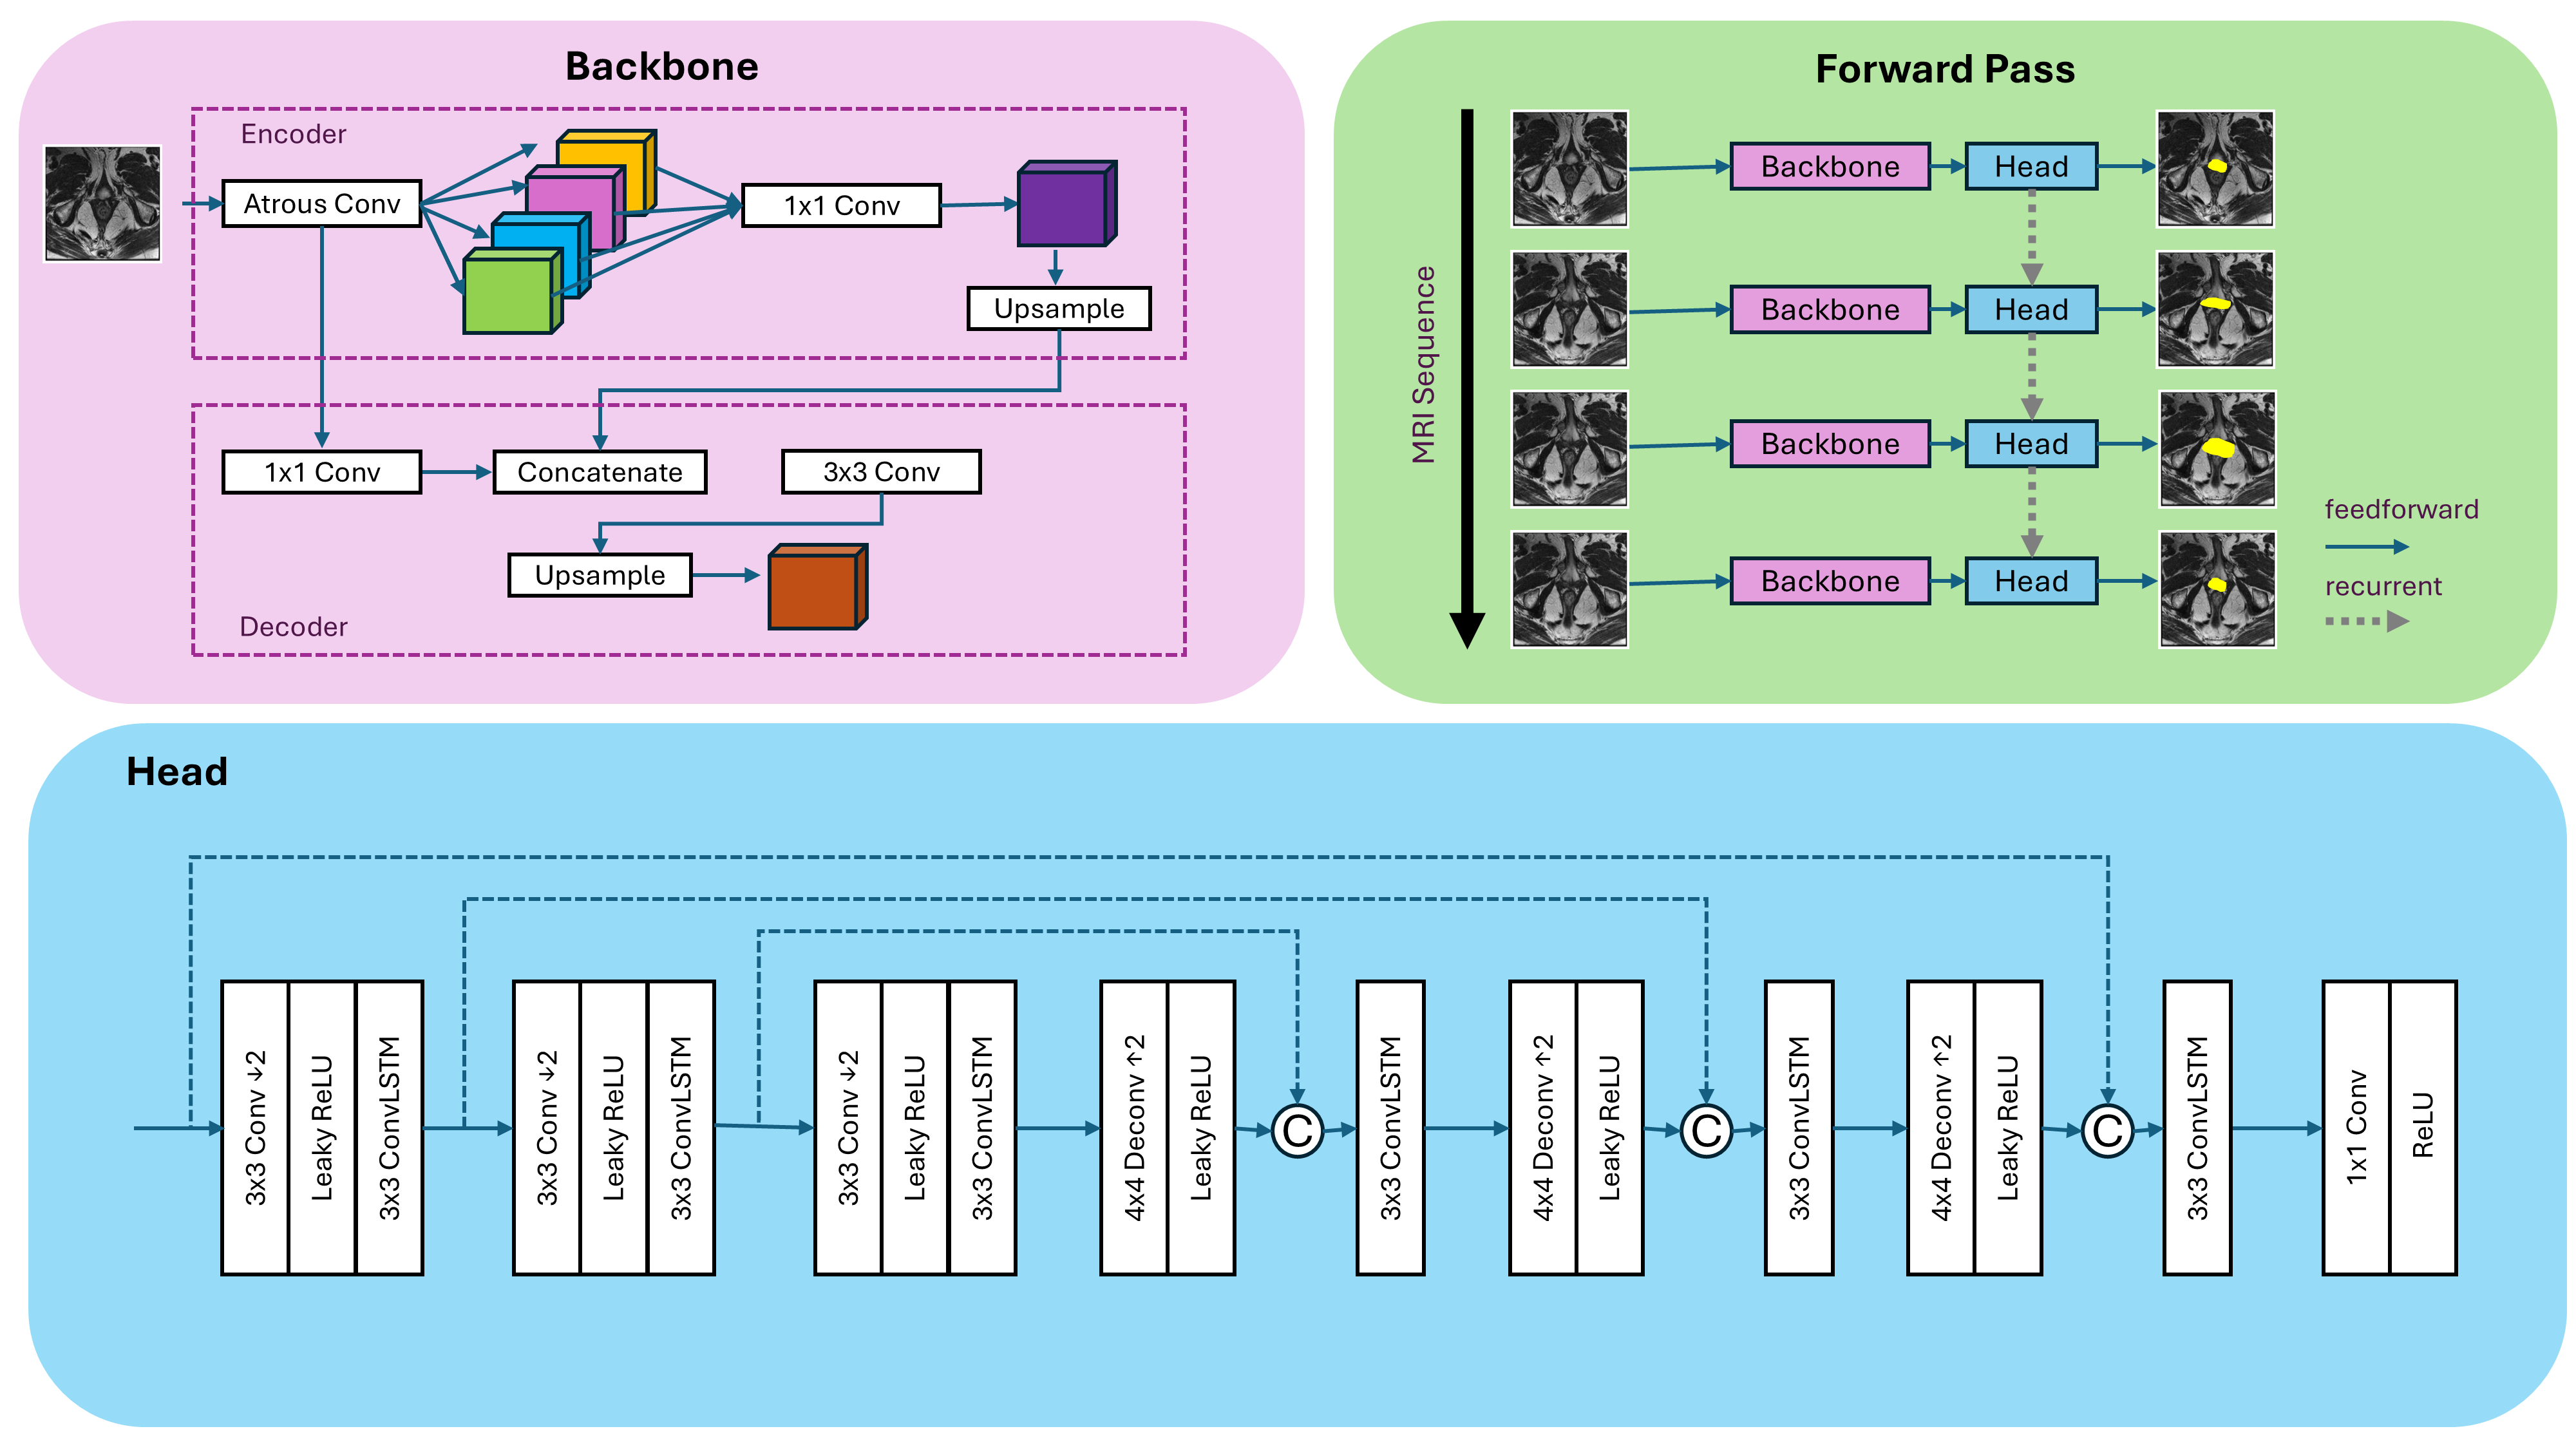
\includegraphics[width=\linewidth]{Fig/architecture.png}
    \caption{Figure shows the inner workings of the proposed model architecture. The backbone consists of DeepLabV3 extracting and aggregating multiscale features from raw MRI slices to produce high level feature maps. For each MRI slice, the backbone's output is further processed by the head to produce the final segmentation map. The head retains memory of past inputs in the activations of its recurrent convolutional layers and uses them in conjunction with feature maps from the current slice to generate its segmentation output. The head consists of regular convolutional layers and recurrent convolutional layers organized in an encoder-decoder configuration. Skip connections from the encoder send its information to the decoder to mitigate the loss of feature resolution in the encoder.}
    \label{fig:architecture}
\end{figure*}

\begin{figure*}
    \centering
    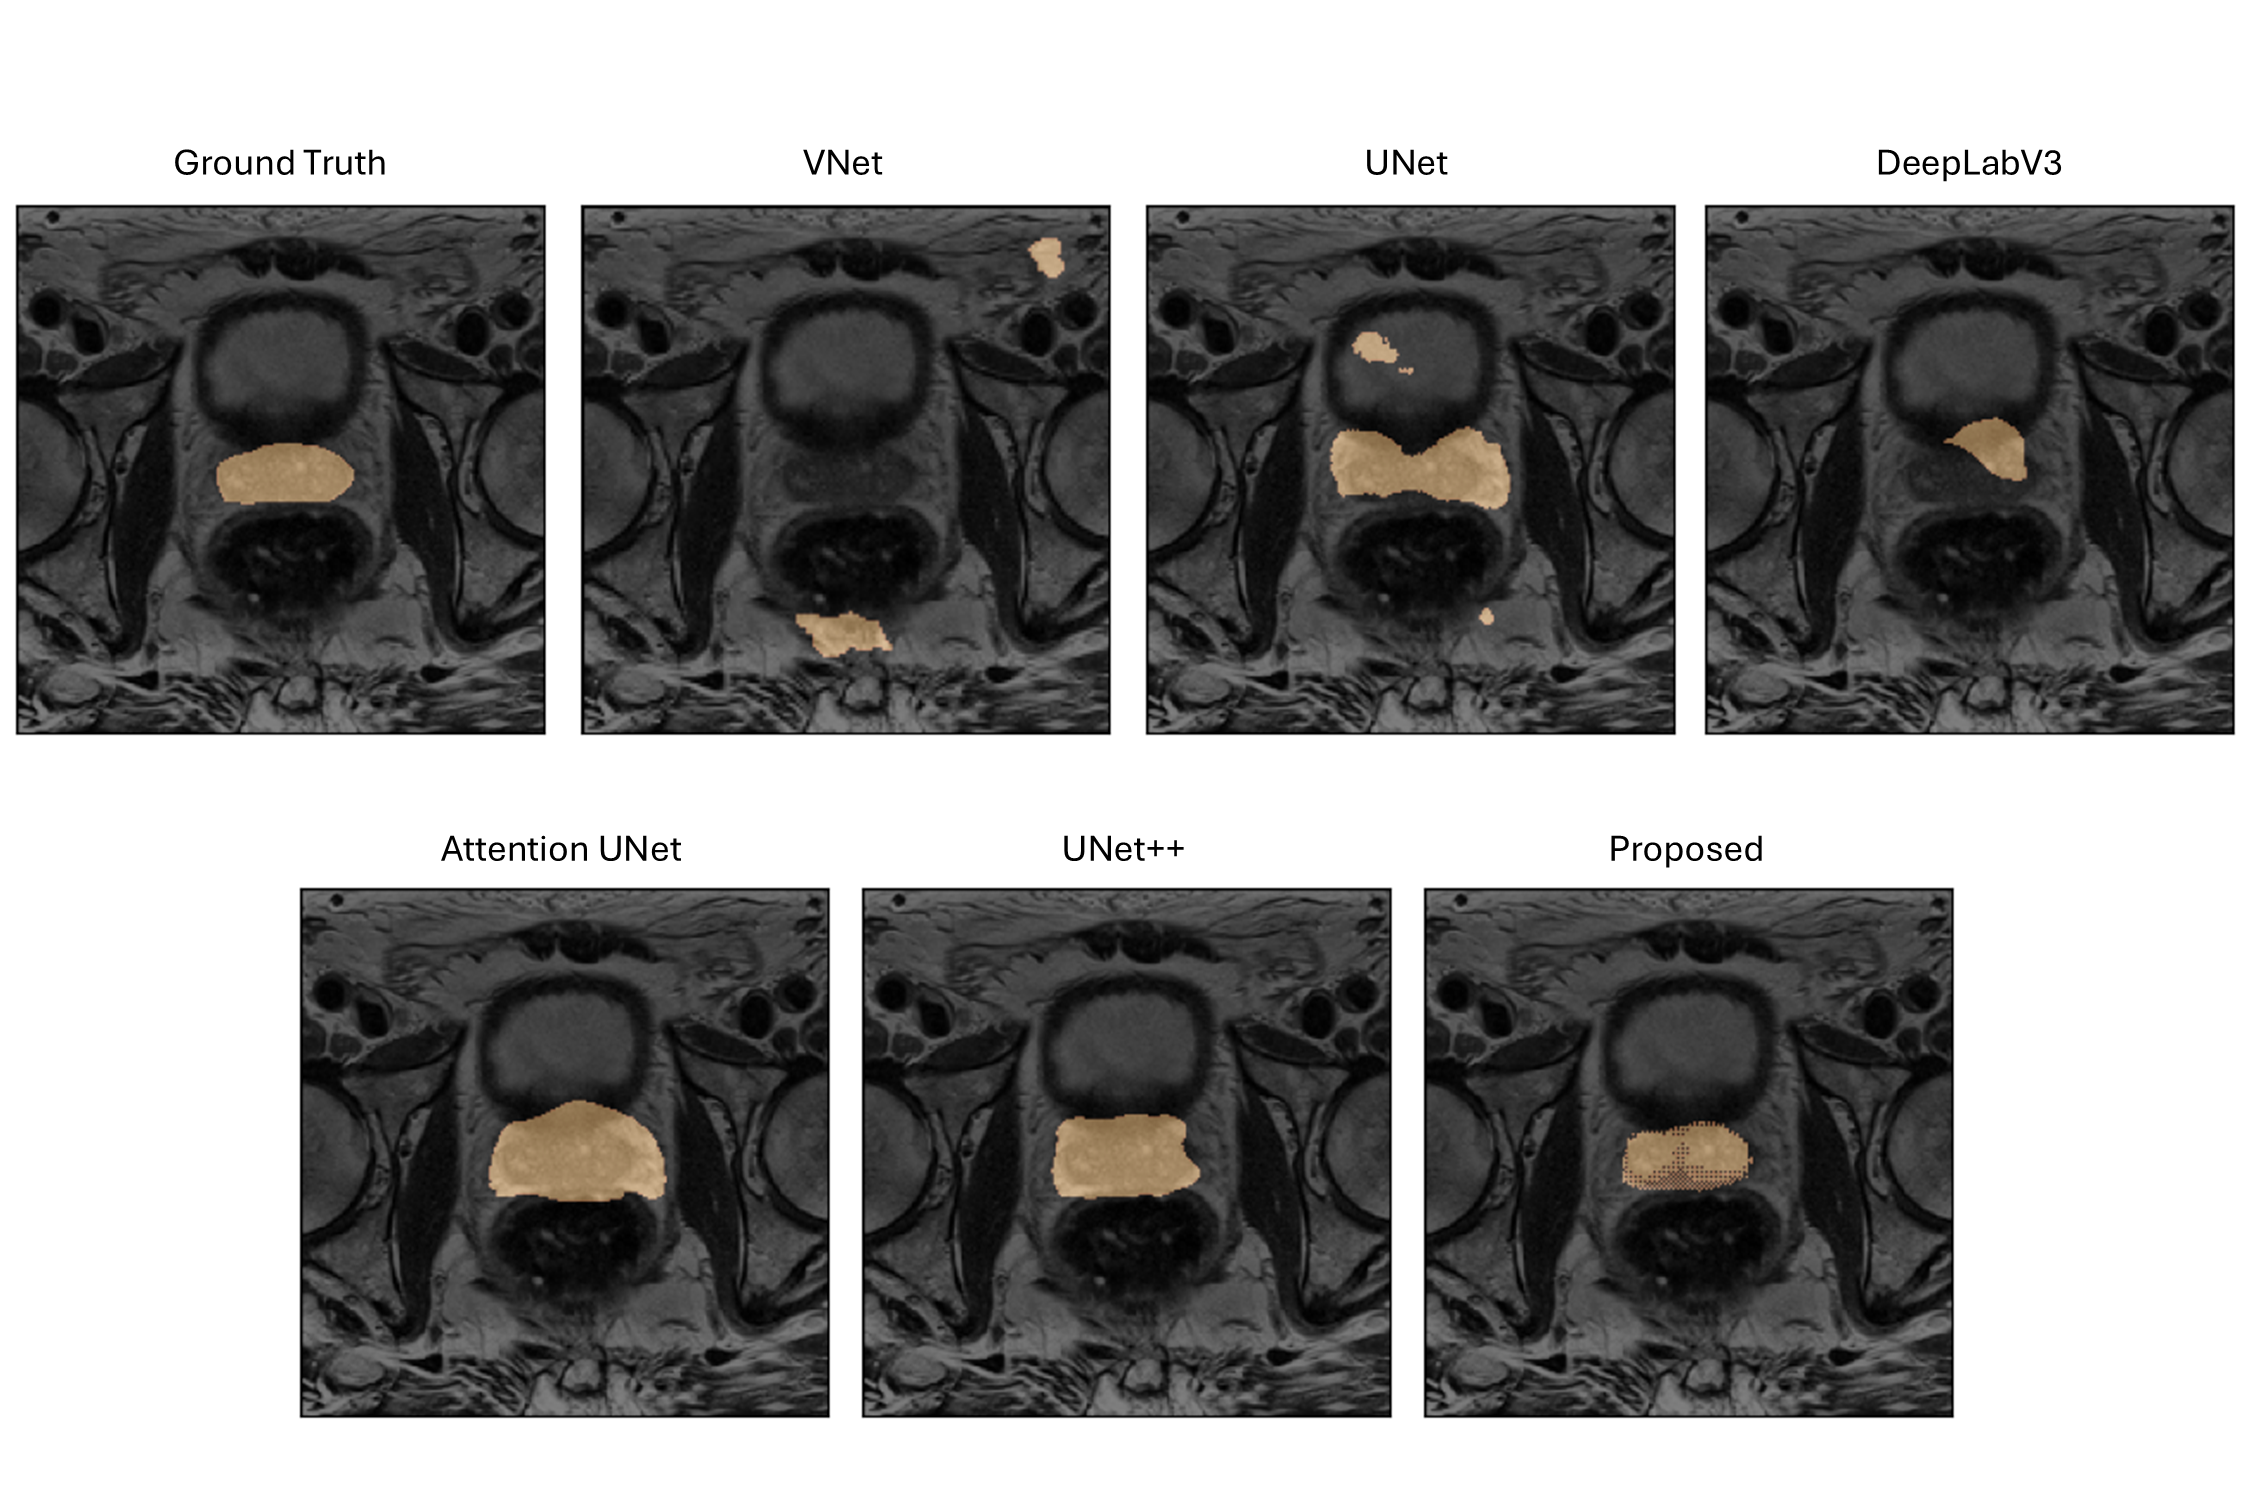
\includegraphics[width=\linewidth]{Fig/patient_7_preds.png}
    \caption{Comparison of segmentation results across various methods compared to the ground-truth (top left). The proposed method (bottom right) can be observed to capture the prostate gland most faithfully compared to benchmark methods.}
    \label{fig:visual}
\end{figure*}


\begin{figure*}
    \centering
    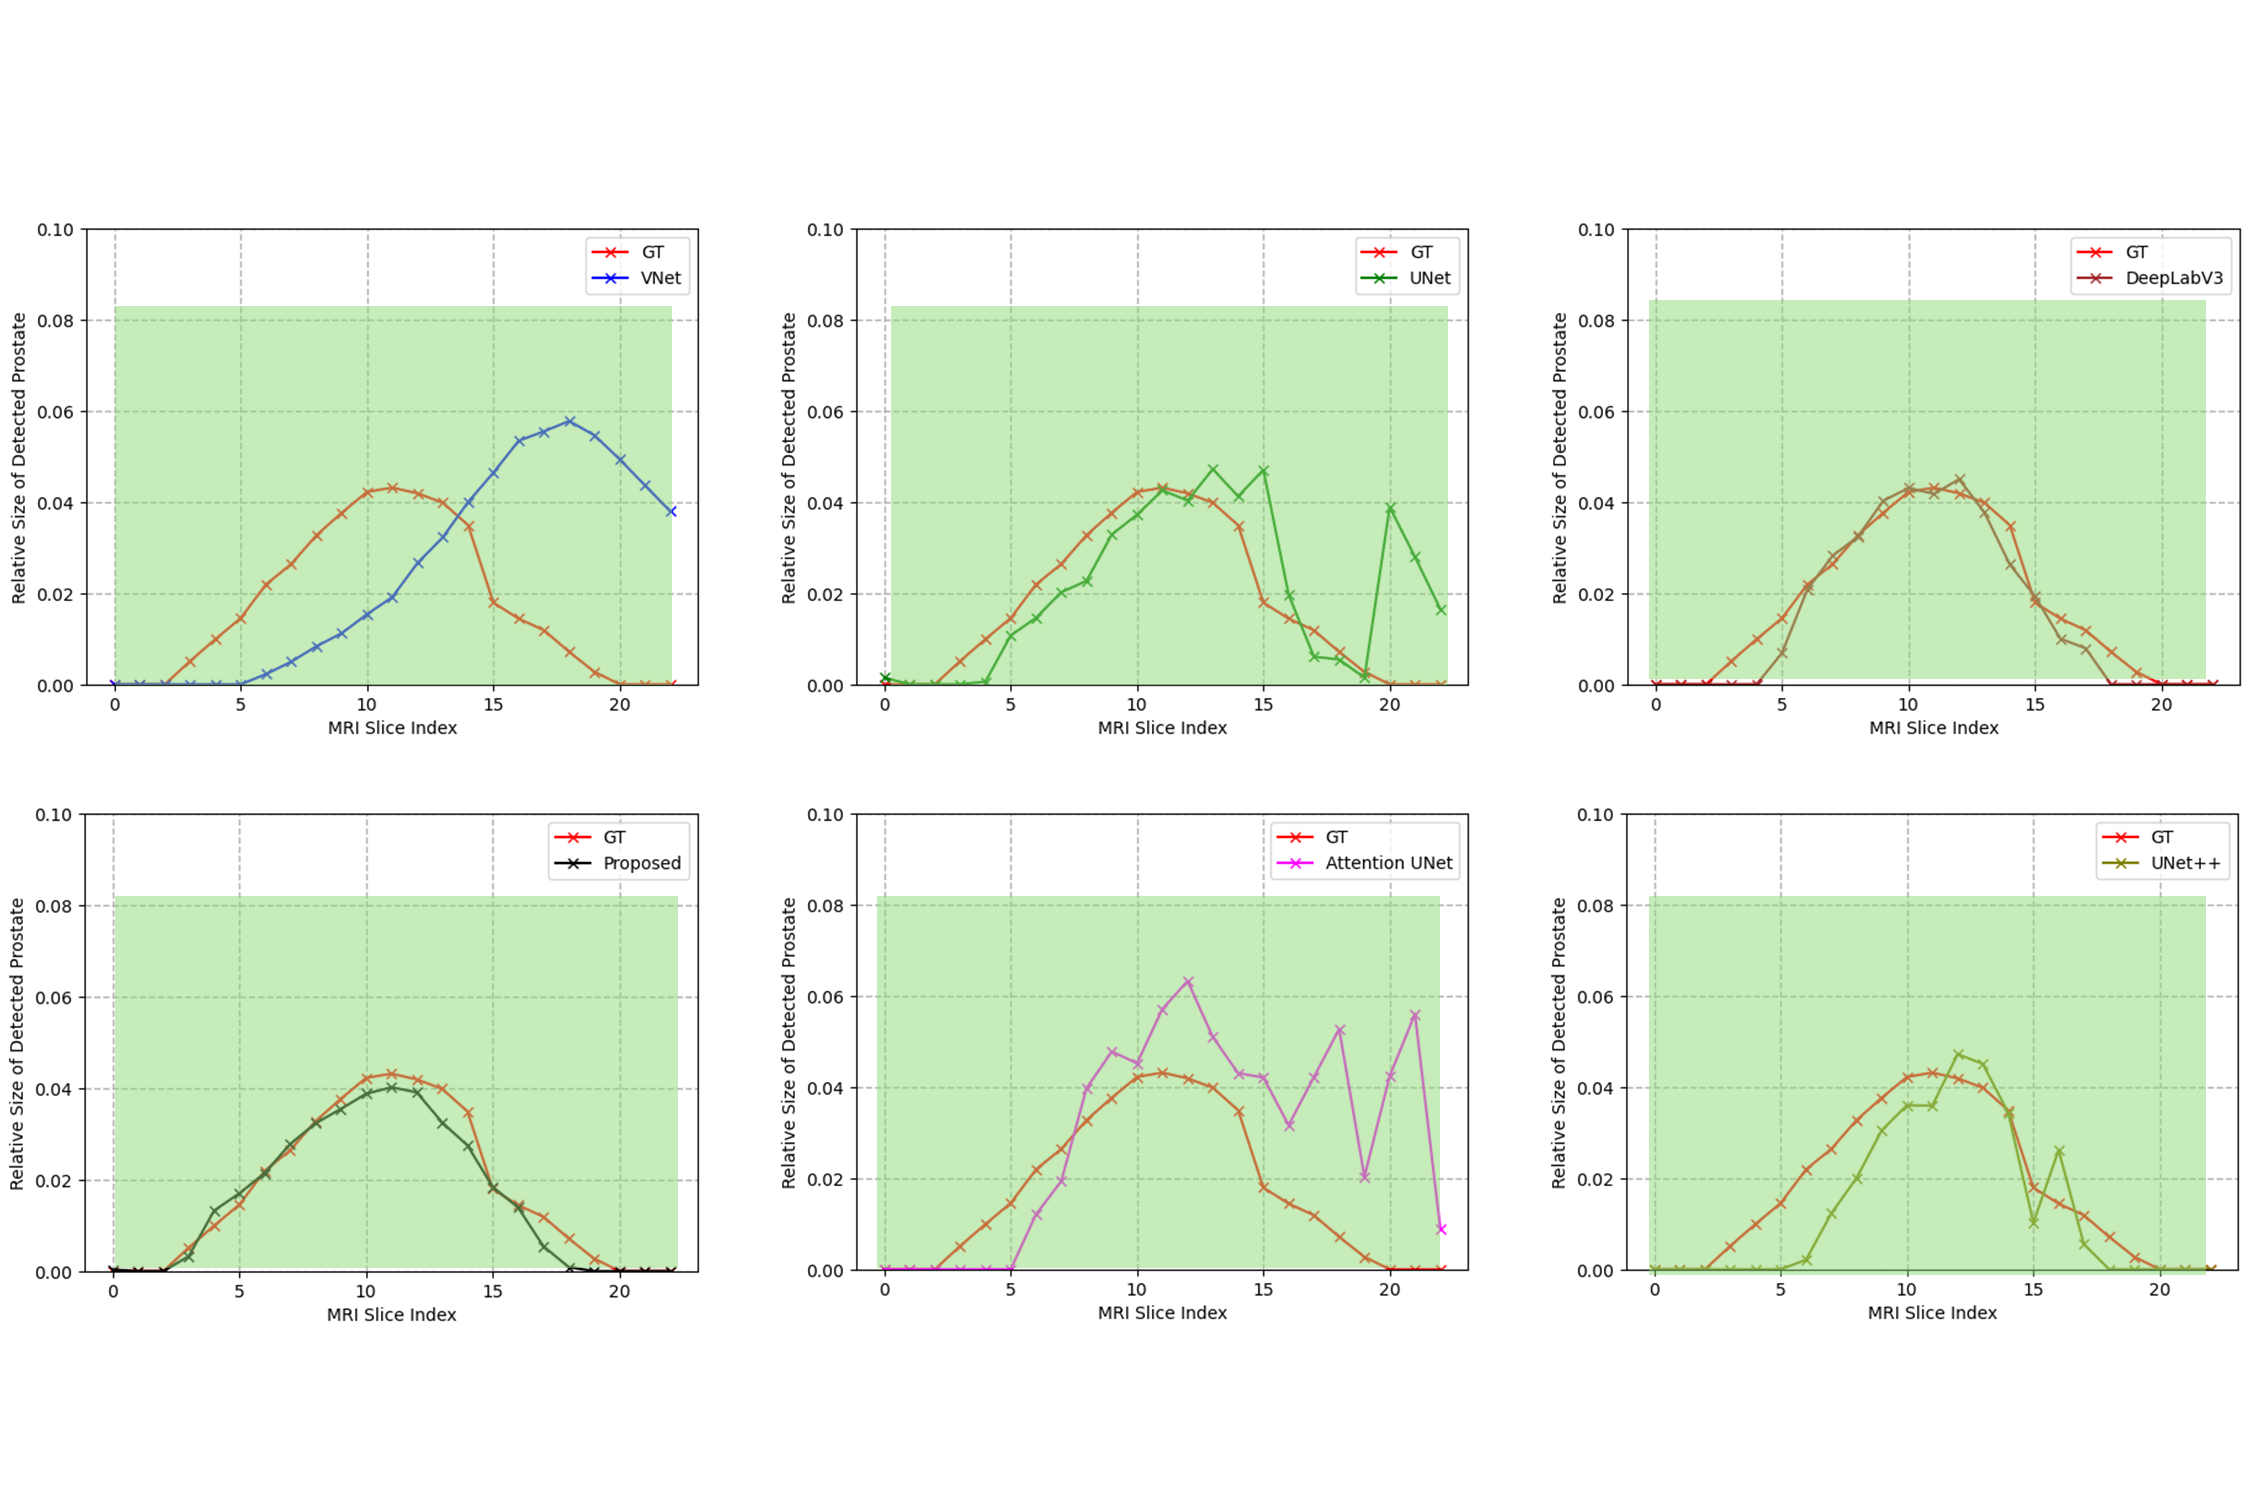
\includegraphics[width=\linewidth]{Fig/patient_4_tumor_profiles_noisefree.png}
    \caption{Comparison of relative prostate sizes (normalized by the image dimensions) across segmentation methods for each MRI slice from a single patient under noise-free imaging conditions (depicted by the green color in the background). Ground-truth measurements are shown alongside predictions from the proposed model and baseline methods from the literature. The predictions of the proposed model (first plot in the second row) can be observed to be best aligned to the reference annotations.}
    \label{fig:patient_4_profiles}
\end{figure*}

\begin{figure*}
    \centering
    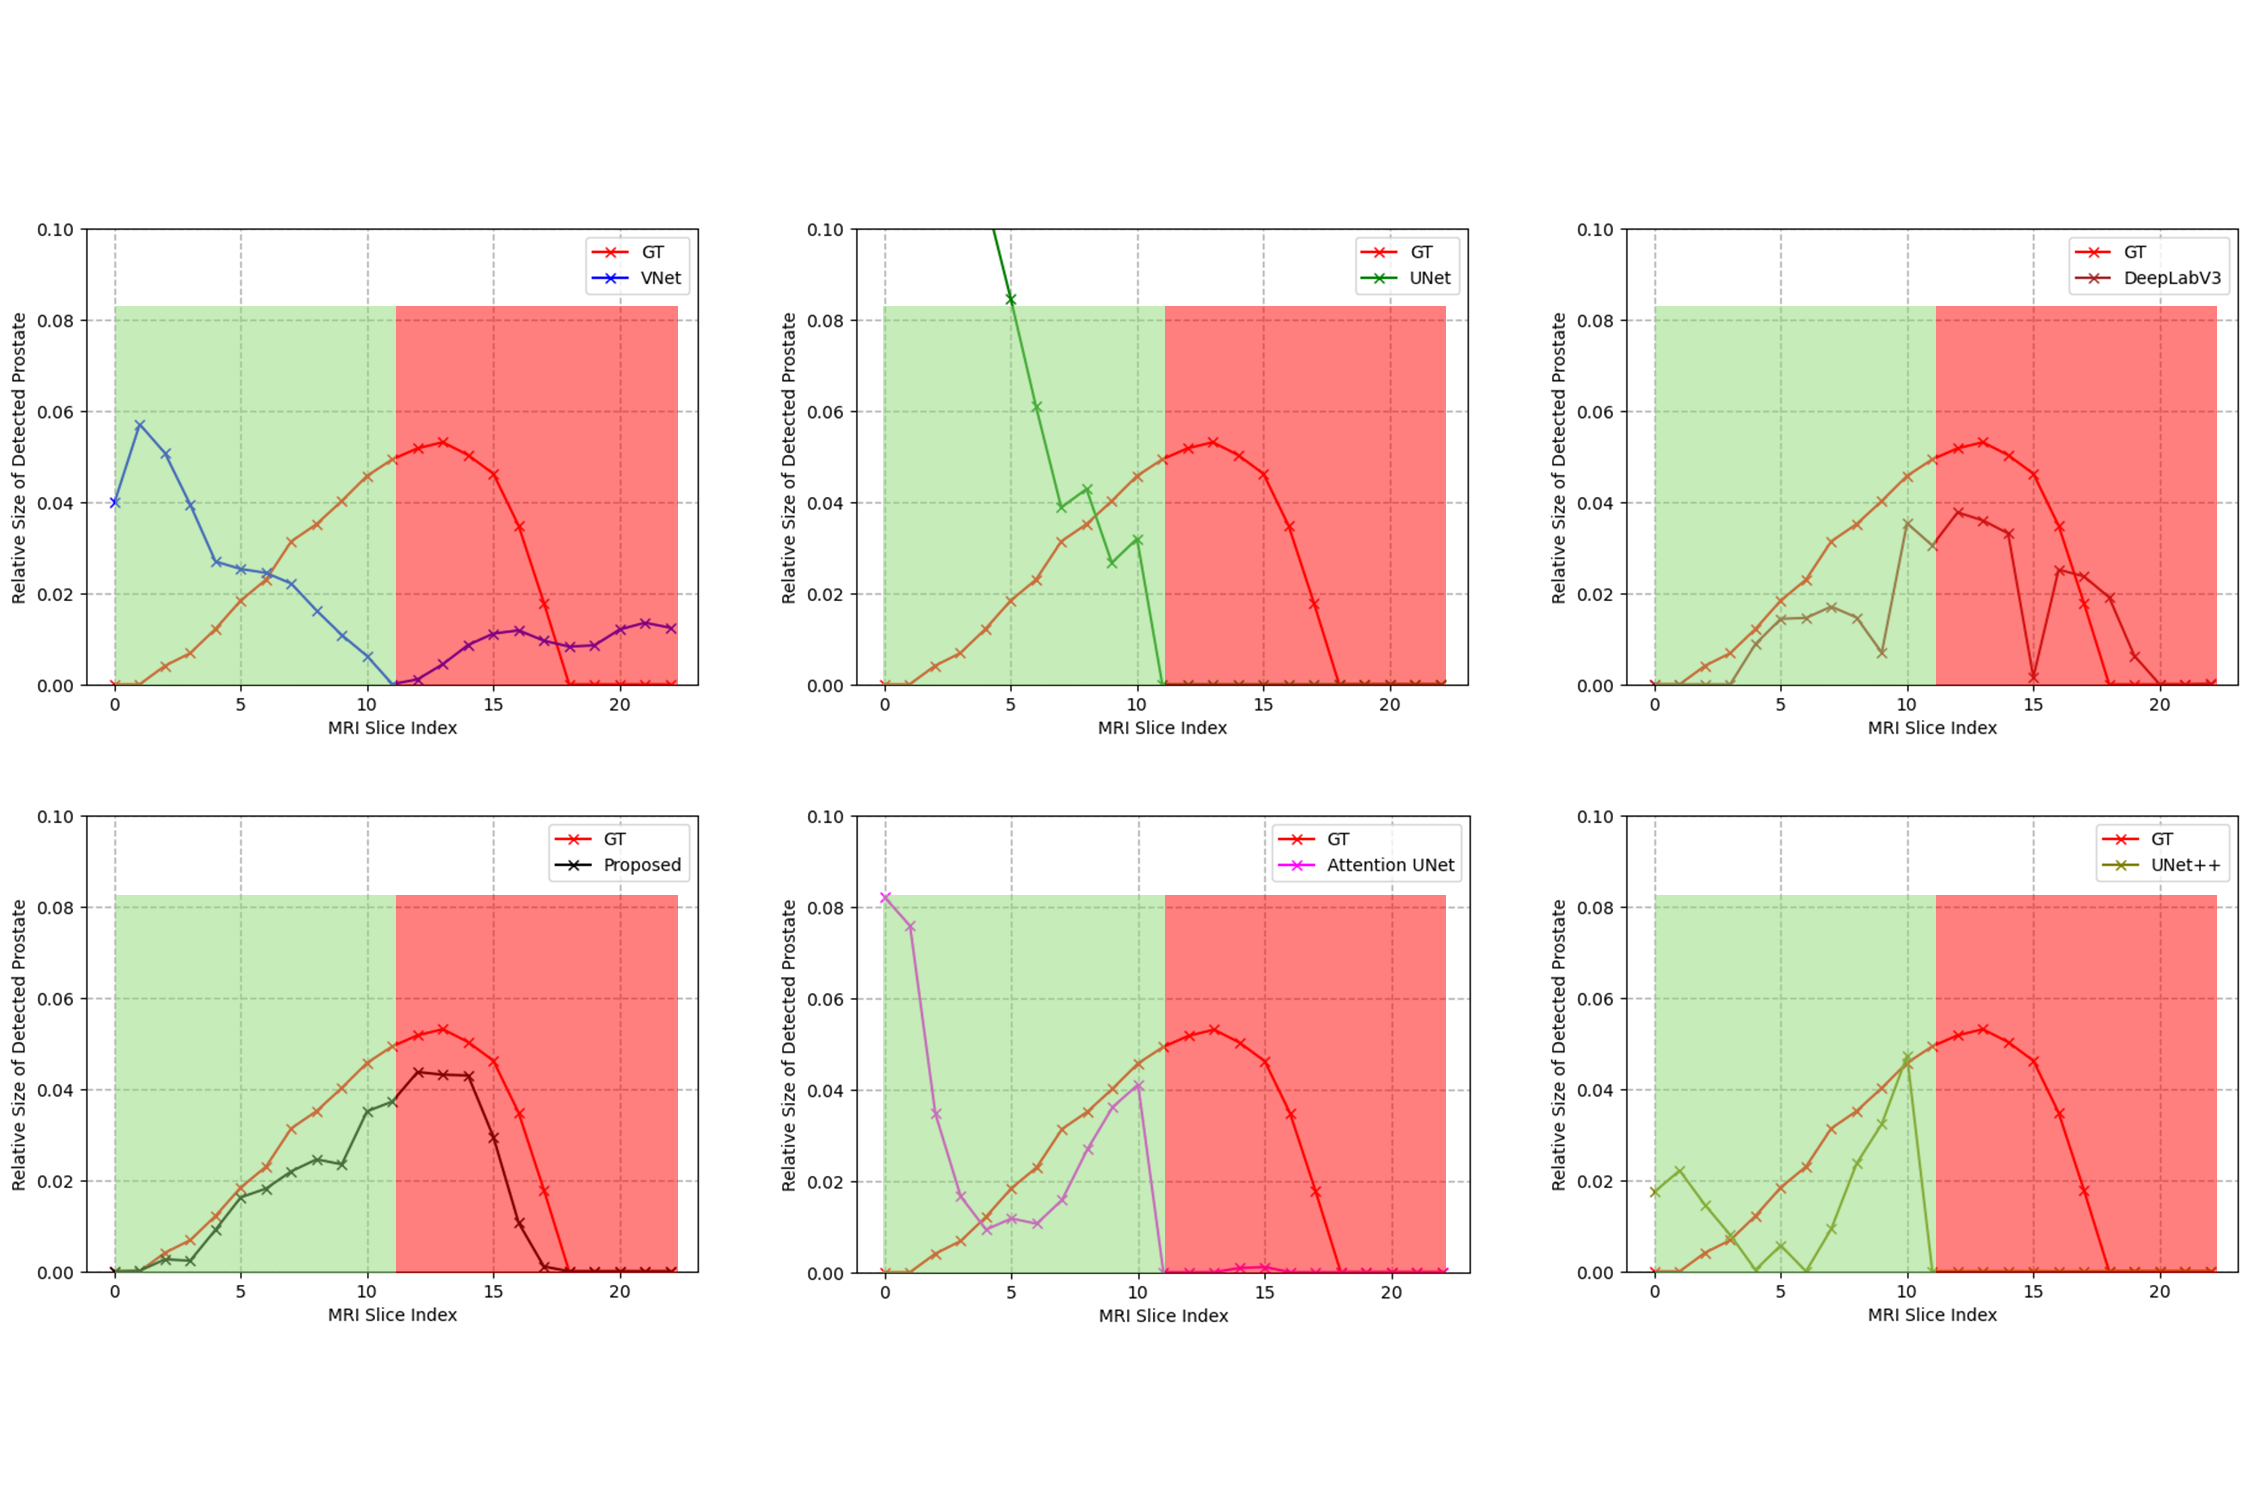
\includegraphics[width=\linewidth]{Fig/patient_2_tumor_profiles.png}
    \caption{Comparison of relative prostate sizes (normalized by the image dimensions) across segmentation methods for each MRI slice from a single patient under noisy imaging conditions. The first half of the sequence (denoted by green) consists of the original noise free images while the second half simulates low contrast imaging into the image slices (denoted by red). Ground-truth measurements are shown alongside predictions from the proposed model and baseline methods from the literature. The proposed model's predictions (first plot on the second row) can be observed to be best aligned to the reference annotations.}
    \label{fig:patient_2_profiles}
\end{figure*}

\begin{table*}[h]
    \centering
    \renewcommand{\arraystretch}{1.3} % Increase row height
    \begin{tabular}{lcccc|cccc}
        \toprule
        \textbf{Architecture} & \textbf{Precision} & \textbf{Recall} & \textbf{F1-score} & \textbf{DSC} & \textbf{Precision} & \textbf{Recall} & \textbf{F1-score} & \textbf{DSC} \\
        \midrule
        & \multicolumn{4}{c}{\textbf{Clean Test Set}} & \multicolumn{4}{c}{\textbf{Corrupted Test Set}}\\
        UNet \cite{ronneberger2015u} & 0.39 & 0.76 & 0.51 & 0.49 & 0.04 & 0.12 & 0.06 & 0.06 \\
        UNet++ \cite{zhou2018unet++} & 0.61 & 0.82 & 0.70 & 0.66 & 0.54 & 0.56 & 0.55 & 0.52\\
        Attention UNet \cite{oktay2018attention}& 0.39 & 0.84 & 0.53 & 0.52 & 0.30 & 0.52 & 0.38 & 0.36\\
        VNet \cite{milletari2016v} & 0.33 & 0.46 & 0.38 & 0.37 & 0.24 & 0.28 & 0.26 & 0.24 \\
        DeepLabV3 \cite{chen2017rethinking} & 0.80 & 0.78 & 0.79 & 0.78 & 0.84 & 0.63 & 0.72 & 0.70\\
        \textbf{Proposed} & \textbf{0.84} & 0.81 & \textbf{0.83} & \textbf{0.82} & \textbf{0.84} & \textbf{0.75} & \textbf{0.79} & \textbf{0.78}\\
        \bottomrule
    \end{tabular}
    \vspace{2mm}
    \caption{Segmentation performance of different architectures on the benchmark dataset.}
    \label{tab:prostate_seg_results}
\end{table*}

\section{Conclusion}
We presented an approach for automatic prostate gland segmentation in T2-weighted MRI sequences leveraging a deep, pretrained segmentation backbone attached to a head comprising recurrent convolutional layers. Our experiments demonstrate that the deep convolutional backbone from the popular DeepLabV3 segmentation model produces robust, generalizable features that are further refined by the recurrent convolutional head to model memory of past input slices in MRI sequences. We benchmarked our approach against a variety of baseline methods in the literature, including the traditional UNet and its various 2D/3D variants. Our proposed method is seen to significantly outperform baseline approaches in limited label settings. Further, our method exhibits considerable resilience to sudden degradations in imaging conditions such as changes in contrast compared to other approaches. Given its robustness to noisy inputs and a high level of generalization in limited label settings, our method shows significant potential for adoption in clinical workflows involving MRI-based prostate localization.


% Can use something like this to put references on a page
% by themselves when using endfloat and the captionsoff option.
\ifCLASSOPTIONcaptionsoff
  \newpage
\fi



% trigger a \newpage just before the given reference
% number - used to balance the columns on the last page
% adjust value as needed - may need to be readjusted if
% the document is modified later
%\IEEEtriggeratref{8}
% The "triggered" command can be changed if desired:
%\IEEEtriggercmd{\enlargethispage{-5in}}

% references section

% can use a bibliography generated by BibTeX as a .bbl file
% BibTeX documentation can be easily obtained at:
% http://mirror.ctan.org/biblio/bibtex/contrib/doc/
% The IEEEtran BibTeX style support page is at:
% http://www.michaelshell.org/tex/ieeetran/bibtex/
\bibliographystyle{IEEEtran}
\bibliography{bibtex/bib/refs}

\appendix
\subsection*{Additional Training Details}
\label{app:training}
All models are trained in PyTorch for 100 epochs with a fixed learning rate of 0.001 using the ADAM optimizer. The MRI sequences in the PROMISE12 dataset exhibit varying sizes. During training and inference, all images are resampled to 224 $\times$ 224 size. Image amplitudes are scaled to lie between 0 and 1. To improve image contrast, histogram equalization is carried out over all slices in the MRI data. 

To keep training costs tractable, we randomly select a subsequence consisting of 10 consecutive slices from the full MRI sequence data of any given patient. For DeepLabV3, UNet, Attention UNet, and UNet++, these slices are ordered in the batch dimension. For the proposed model, these image slices are processed image-wise by the backbone. Thereafter, the output of the backbone is rearranged so that the respective feature maps for each image slice form a sequence to be input to the recurrent convolutional head. Since inference requires less GPU VRAM, each MRI sequence is processed as a whole (versus subsamples of size 10 as in training). For VNet, each subsequence is padded to a standard size of 96 in the sequence length dimension to allow processing by the full depth of the model. However, the loss is only computed for the first 10 slices to prevent padded slices from contributing to the backpropagated gradients.   Both training and inference is carried out on a single NVIDIA T4 GPU featuring 16GB of GPU VRAM.  




% biography section
% 
% If you have an EPS/PDF photo (graphicx package needed) extra braces are
% needed around the contents of the optional argument to biography to prevent
% the LaTeX parser from getting confused when it sees the complicated
% \includegraphics command within an optional argument. (You could create
% your own custom macro containing the \includegraphics command to make things
% simpler here.)
%\begin{IEEEbiography}[{\includegraphics[width=1in,height=1.25in,clip,keepaspectratio]{mshell}}]{Michael Shell}
% or if you just want to reserve a space for a photo:

% \begin{IEEEbiography}{Michael Shell}
% Biography text here.
% \end{IEEEbiography}

% % if you will not have a photo at all:
% \begin{IEEEbiographynophoto}{John Doe}
% Biography text here.
% \end{IEEEbiographynophoto}

% % insert where needed to balance the two columns on the last page with
% % biographies
% %\newpage

% \begin{IEEEbiographynophoto}{Jane Doe}
% Biography text here.
% \end{IEEEbiographynophoto}

% You can push biographies down or up by placing
% a \vfill before or after them. The appropriate
% use of \vfill depends on what kind of text is
% on the last page and whether or not the columns
% are being equalized.

%\vfill

% Can be used to pull up biographies so that the bottom of the last one
% is flush with the other column.
%\enlargethispage{-5in}



% that's all folks
\end{document}

Use \cite{Fassia2024}

Use \cite{turkbey2022deep}

Use \cite{LUNDERVOLD2019102}

Use \cite{shamshad2023transformers}

others: \cite{pozaruk2021augmented}
